\documentclass[11pt, brazil, a4paper, usenames, svgnames, dvipsnames]{article}
\usepackage[brazil]{babel}
\selectlanguage{brazil}
\usepackage[T1]{fontenc}
\usepackage[utf8]{inputenc}
\usepackage[usenames,svgnames,dvipsnames]{xcolor}
%\usepackage[latin1]{inputenc}
%\usepackage[iso-8859-7]{inputenc}
\usepackage{url}
\usepackage{lscape}
\usepackage{tabularx}
\usepackage{longtable}
\usepackage{setspace}
\usepackage[pdftex]{graphicx}
\usepackage{mathtools}
\usepackage{bm}
\usepackage{pdfpages}
\usepackage{placeins}
\usepackage{indentfirst}

% \usepackage{helvet}
% \renewcommand{\familydefault}{\sfdefault}
\usepackage{color}

%\usepackage{indentfirst}                % indentação do primeiro parágrafo

%\setlength{\oddsidemargin}{-2mm}
%\setlength{\evensidemargin}{-2mm}
%\setlength{\textwidth}{160mm}
%\setlength{\textheight}{200mm}
%\setlength{\topmargin}{-3mm}
\setlength{\parskip}{2mm}
\usepackage[a4paper,top=3cm,bottom=3cm,left=3cm,right=2cm]{geometry} %

%\linespread{1.3}

%\usepackage[round,sort,nonamebreak]{natbib} % 
%\bibpunct{(}{)}{;}{a}{,}{,}

\usepackage{fancyhdr}
\pagestyle{fancy}

% ------------------------------------------------------------------ %
%\usepackage[usenames,svgnames,dvipsnames]{xcolor}

%\usepackage[format=plain,labelfont=bf,up,textfont=it,up]{caption}
\usepackage[font=small,format=plain,labelfont=bf,up,textfont=it,up]{caption}

\usepackage[pdftex,plainpages=false,pdfpagelabels,
	linktocpage,
	letterpaper,
	colorlinks=true,
	citecolor=DarkGreen,
	linkcolor=NavyBlue,
	urlcolor=DarkRed,
	filecolor=green,
	bookmarksopen=true
]{hyperref}



%\onehalfspacing  % espaçamento
\singlespacing  % espaçamento

% ------------------------------------------------------------------ %
%\setlength\headheight{92pt} 
\lhead{F. Costa, R. Oliveira, V. Barros}
\rhead{Projeto de Algoritmos e Estruturas de Dados I}


\title{Benchmark de Algoritmos de Ordenação:\\Projeto de Algoritmos e Estruturas de Dados I}

\author{Felipe Anchieta Santos Costa \\ Rodrigo Martins de Oliveira\\ Victor Campagner de Barros\\\\ \\ {Bacharelado em Ciência da Computação}\\ {Universidade Federal do ABC}\\ }
\date{Santo André, 29 de abril de 2015}

\begin{document}

\maketitle

% ------------------------------------------------------------------ %
\begin{abstract}
\parindent=3cm
O presente trabalho, através de algoritmos eficientes e ineficientes de ordenação de vetores de inteiros implementados em C++, apresenta os gráficos de execuções desses algoritmos em vetores de tamanhos pré-estabelecidos preenchidos com números pseudoaleatórios. Desta forma, concluimos sobre a abordagem de ordenação mais eficiente.
\\
\\
\noindent
Palavras-chave: Algoritmos. Ordenação. Benchmark.
\end{abstract}

\newpage

\noindent
\section{Introdução}
\label{sec:introducao}
\hfill

%\parindent=3cm
O uso de vetores de dados é comum à todas as áreas do conhecimento e, por vezes,
é necessário extrair informações destes ou simplesmente ordená-lo segundo um
critério conveniente.

Quando se trabalham com um volume de dados muito grande,
muitos vetores e/ou vetores de muitos elementos o auxílio de um algoritmo
computacional pode ser desejável ou necessário para realizar operações sobre
o vetor e/ou extrair informações deste.

Independe do propósito para o qual se
utilizará o vetor, é conveniente que este esteja ordenado, pois sabendo que
os elementos seguem alguma ordem, a busca de informações neste vetor será mais
eficiente. O problema de ordenação de vetores é bem conhecido e estudado na literatura e
existem diversos algoritmos para tal.

A análise e comparação destes algoritmos é feita através da análise da complexidade
deste e, também, da realização de benchmarks.

A função de complexidade de um algoritmo fornece o comportamento do algoritmo sobre
a variação de um parâmetro relevante. Para algoritmos de ordenação, este parâmetro é
o tamanho dos vetores a serem ordenados. Relacionando o número de comparações realizadas
conforme o tamanho dos vetores varia fornece o número de comparações em função do tamanho
da entrada. Com esta informação extrai-se a ordem de complexidade do algoritmo. 

Para um algoritmo, geralmente, se analisa a complexidade de três casos específicos:
melhor caso, caso médio e pior caso. E com os dados obtidos se escrevem a ordem de
complexidade do algoritmo nestes casos em notação assintótica. Neste notação $\Omega(g(n))$
denota o compartamento no melhor caso, $O(g(n))$, o comportamento no pior caso e $\Theta(g(n))$ para
denotar que o melhor e pior caso são os mesmos, ou para indicar o comportamento em um
caso específico, como o caso médio.

A realização de um benchmark, isto é, de um teste empírico, baseado no tempo de
execução de um algoritmo é útil para comparar facilmente dois ou mais algoritmos
em casos específicos e também é um meio de garantir que o algoritmo tem o comportamento
esperado obtido através da análise de sua complexidade.

Neste projeto será realizado um benchmark dos algoritmos de ordenação expostos na
disciplina Algoritmos e Estruturas de Dados I, ministrada pelo professor André Balan.
Os resultados de cada algoritmo serão comparados para analisar o desempenho de cada
um em relação aos demais e asseverar os conceitos aprendidos na disciplina.

\noindent
\section{Objetivos}

\hfill

\begin{itemize}
\item Implementar os algoritmos de ordenação propostos;
\item Realizar um benchmark dos algoritmos implementados;
\item Comparar os algoritmos através dos resultados do benchmark.
\end{itemize}

\noindent
\section{Metodologia} \label{metodologia}

\hfill

Os algoritmos considerados neste trabalho foram implementados em C++ de forma
a receberem \textit{arrays} de elementos de quaisquer tipos. Além das funções
específicas de cada método de ordenação, foram criadas funções para gerar
vetores aleatórios a partir da utilização de um cabeçalho indicado pelo professor
André Balan, verificar se um vetor estava ordenado de forma crescente, registrar
o tempo de execução dos algoritmos e imprimir os resultados para um arquivo CVS\footnote{Do inglês: \emph{Comma-separated values}}.

Para fornecer uma amostra razoável de dados, cada algoritmo foi testado com 6
vetores diferentes para cada tamanho considerado. Os algoritmos descritos na
literatura como eficientes foram testados com um conjunto de tamanhos para os
vetores que compreendia o intervalo $[10000,65610000]$, já os algoritmos descritos
como ineficientes foram testados com um conjunto que compreendia um valor máximo menor
do que o intervalo anterior, $[10000,150000]$.

Os algoritmos considerados neste trabalho foram: Bubble Sort, Insert Sort, Select Sort, Quick Sort, Heap Sort, Shell Sort, Merge Sort, {\ttfamily qsort} da biblioteca padrão da linguagem C e {\ttfamily sort} da biblioteca padrão da linguagem C++. Destes, Bubble Sort, Insert Sort e Select Sort são descritos na literatura como métodos de ordenação ineficientes, enquanto que os outros são considerados eficientes.

Através da realização do benchmark dos algoritmos supracitados eles foram comparados. No resto desta seção são descritos brevemente cada um dos algoritmos considerados.

\subsection{Bubble Sort}
Este método de ordenação é considerado um dos mais simples existentes e consiste
na comparação de pares de elementos consecutivos. O algoritmo inicia comparando o
primeiro elemento do vetor com seu consecutivo até comparar o penúltimo com seu
consecutivo. Quando um elemento é maior do que seu consecutivo, suas posições são
trocadas e avança-se um elemento para realizar a próxima comparação. Ao final do processo
o maior elemento do vetor estará na posição correta e então se repete o processo para que
o segundo maior elemento esteja na posição correta e assim por diante até que o vetor
esteja completamente ordenado. Este método é considerado ineficiente, pois apresenta
complexidade $O(n^2)$ e $\Omega(n)$, ou seja, ele se comporta de maneira linear em relação ao
número de comparações realizadas conforme aumenta o número de elementos do vetor no melhor caso,
e apresenta um comportamento quadrático no pior caso.

\subsection{Quick Sort}
O método de ordenação Quicksort, um dos mais populares métodos de ordenação utilizados hoje em dia, consiste na escolha de um pivô e coloca todos os números maiores que o ele à sua direita e todos os menores à sua esquerda. Ao fazer isso, chama-se recursivamente o algoritmo para a parte da direita e para a da esquerda, organizando novamente em volta de um pivô e chamando recursivamente até que a chamada tenha tamanho 1.
Cada pivô já está em sua posição correta no vetor, e a cada chamada recursiva realizada, ``fixa-se'' um elemento e sua posição correta.
O algoritmo tem tempo no pior caso $O(n^2)$, e mesmo assim é um dos algoritmos mais utilizados pois tem tempo médio de O(nlogn) com boa estabilidade.
\subsection{Merge Sort}

O método Mergesort conhecido como \textit{Divide and Conquer} basicamente divide o vetor principal de tamanho \textbf{n} em pequenos vetores de tamanho \textbf{n/2} recursivamente até que cada um deles tenha tamanho 1. Depois de todas as divisões ele volta um a um em cada recursão e organiza os elementos em ordem crescente pegando sempre o menor valor dentre os vetores restantes em tempo $O(n)$. O algoritmo tem tempo $O(n \log{n})$, tempo considerado o ideal para ordenações baseadas em comparações.
\noindent

\subsection{Heap Sort}

O Heapsort é um algoritmo de ordenação que foge do tradicional. Ao invés de trabalhar com um vetor e tentar ordená-lo, o método cria uma árvore binária chamada heap e organiza os elementos ao inserí-los um a um na estrutura. Com a organização final da heap, tem-se uma disposiçao de maior para menor seguindo da raiz para as folhas, tornando simples o processo de devolver o vetor em ordem. O algoritmo tem tempo $O(n \log{n})$.


\subsection{Insertion Sort}


O insertion sort é um algoritmo considerado eficiente para pequenos tamanho de entrada, mas pouco eficiente de acordo com o aumento desta. Ele inicia no segundo elemento e vai voltando ao início do vetor, enquanto leva o elemento até a menor posição. Em seguida, segue-se ao próximo elemento e caminha-se pela região ordenada até achar um número menor que ele. Ele tem tempo $O(n^2)$ em seu pior e médio caso. Para o melhor caso, ele tem tempo $O(n)$, sendo o algoritmo mais rápido em casos onde o vetor já está ordenado.

\subsection{Shell Sort}

O algoritmo Shell Sort funciona de maneira similiar ao Insert Sort, porém introduzindo
``saltos'' grandes na troca de elementos.

Basicamente, este método considera subsequências
dentro do vetor, não contíguas, compostas de elementos espaçados segundo uma constante $k$.

A primeira subsequência começa no índice $0$ e avança de $k$ em $k$ elementos, nesta subsequência
o algoritmo executa o procedimento de ordenação do Insert Sort e repete este processo para a
próxima subsequência iniciada um indíce após a anterior e mantendo o mesmo espaçamento, até que
que o índice inicial da sequência seja igual ao segundo índice da primeira sequência.

Após esta etapa os elementos do vetor estarão semi-ordenados, isto é, estarão perto da
posição correta com um erro de, no máximo, $k-1$ posições.

O algoritmo se repete considerando $k$'s cada vez menores até que $k=1$. A escolha das constantes
$k$ é o que torna o algoritmo eficaz ou não. Em 1959 Donald Shell, que propôs o algoritmo Shell Sort
utilizou a sequência $n/2, n/4, n/8, \ldots$, onde $n$ é o tamanho do vetor, para determinar
os valores de $k$. A eficiencia destas escolhas para $k$ conferia ao Shell Sort complexidade
$O(n)$.

Uma sequência mais eficiente para obter valores de $k$ foi proposta
por Donal Knuth, onde $k$ segue os valores da sequência $(n-1)/3, (n-1)/9, (n-1)/27, \ldots$.
Para estes valores de $k$ a eficiência do Shell Sort foi melhorada para $O(n \log{n})$.

Porém foi com a sequência proposta por Neils Pardon, em 2009, que o Shell Sort
atingiu a melhor eficiência. Nesta sequência são tomados números de Fibonacci,
deixando de fora o primeiro '1' da sequência, elevando-os à potência de 2 vezes
a proporção áurea. Escolhe-se o maior $k$ possível desta sequência e então se
seguem os $k$ cada vezes menores da sequência até $k=1$. A complexidade do Shell
Sort continua sendo $O(n \log{n})$, porém empiricamente estas escolhas para $k$ demonstram
um melhor desempenho do que qualquer outra escolha já testada na literatura.

Neste projeto os valores de $k$ para o Shell Sort foram escolhidos segundo a
sequência proposta por Pardons.


\subsection{Selection Sort}

O Selection Sort é um algoritmo pouquíssimo utilizado pois tem tempo de execução em seu melhor caso de $O(n^2)$. Ele consiste em achar o menor elemento do vetor e deixá-lo na posição 0. Em seguida procura o menor elemento do vetor restante e aloca-o na posição 1, e assim por diante até que o vetor esteja ordenado. O problema da técnica é que para toda ordenação, obrigatoriamente o algoritmo percorrerá todo a região do vetor não ordenada \textbf{n} vezes.


\subsection{Introsort}

O Introsort, demonstrado nos resultados como Sort C, é um algoritmo híbrido, utilizado nativamente pelo C++. O quicksort é a primeira tentativa do algoritmo em tentar ordenar o vetor, mas quando percebe-se uma falta de eficiência devido ao alto número de chamadas recursivas, o Introsort troca o método de ordenação para o Heapsort, que tem $O(n \log{n})$ mesmo em seu pior caso.

\section{Resultados}

\hfill

Os resultados do benchmark estão apresentados a seguir em forma de gráficos. No
Gráfico \ref{chart:comp_inefic} os algoritmos ineficientes são comparados; no
Gráfico \ref{chart:comp_efic} os algoritmos eficientes são comparados; e no Gráfico
\ref{chart:comp_todos} todos os algoritmos são comparados.  

\noindent

\begin{figure}[hb]
	\centering
	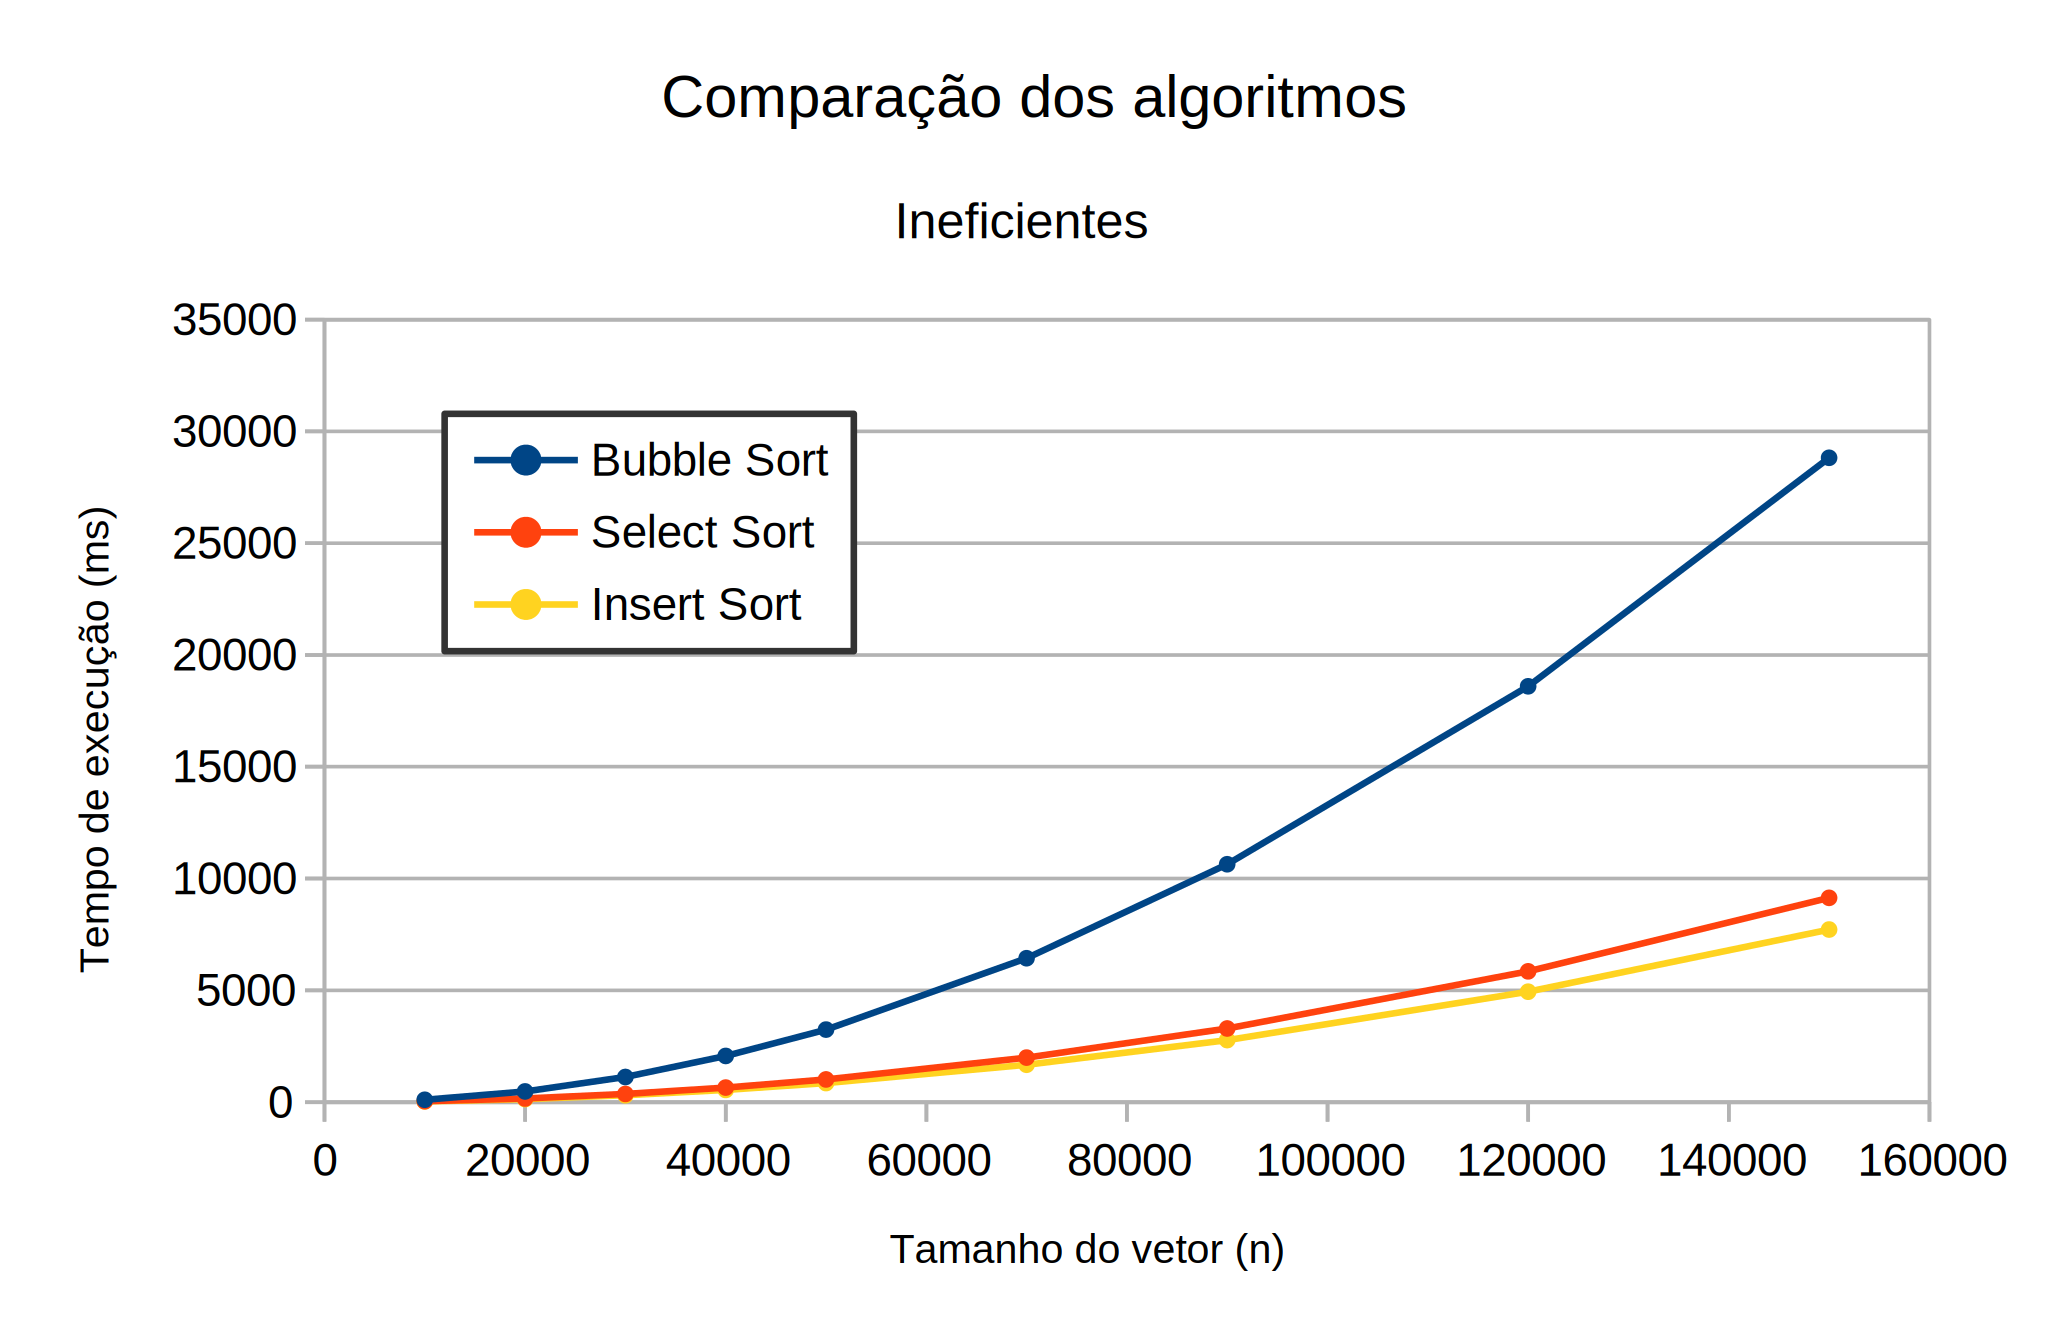
\includegraphics[width=10cm]{comp_inefic.png}
	\caption[Comparação dos algoritmos ineficientes.]
	{Comparação dos algoritmos ineficientes.}
	\label{chart:comp_inefic}
\end{figure}

\begin{figure}[hb]
	\centering
	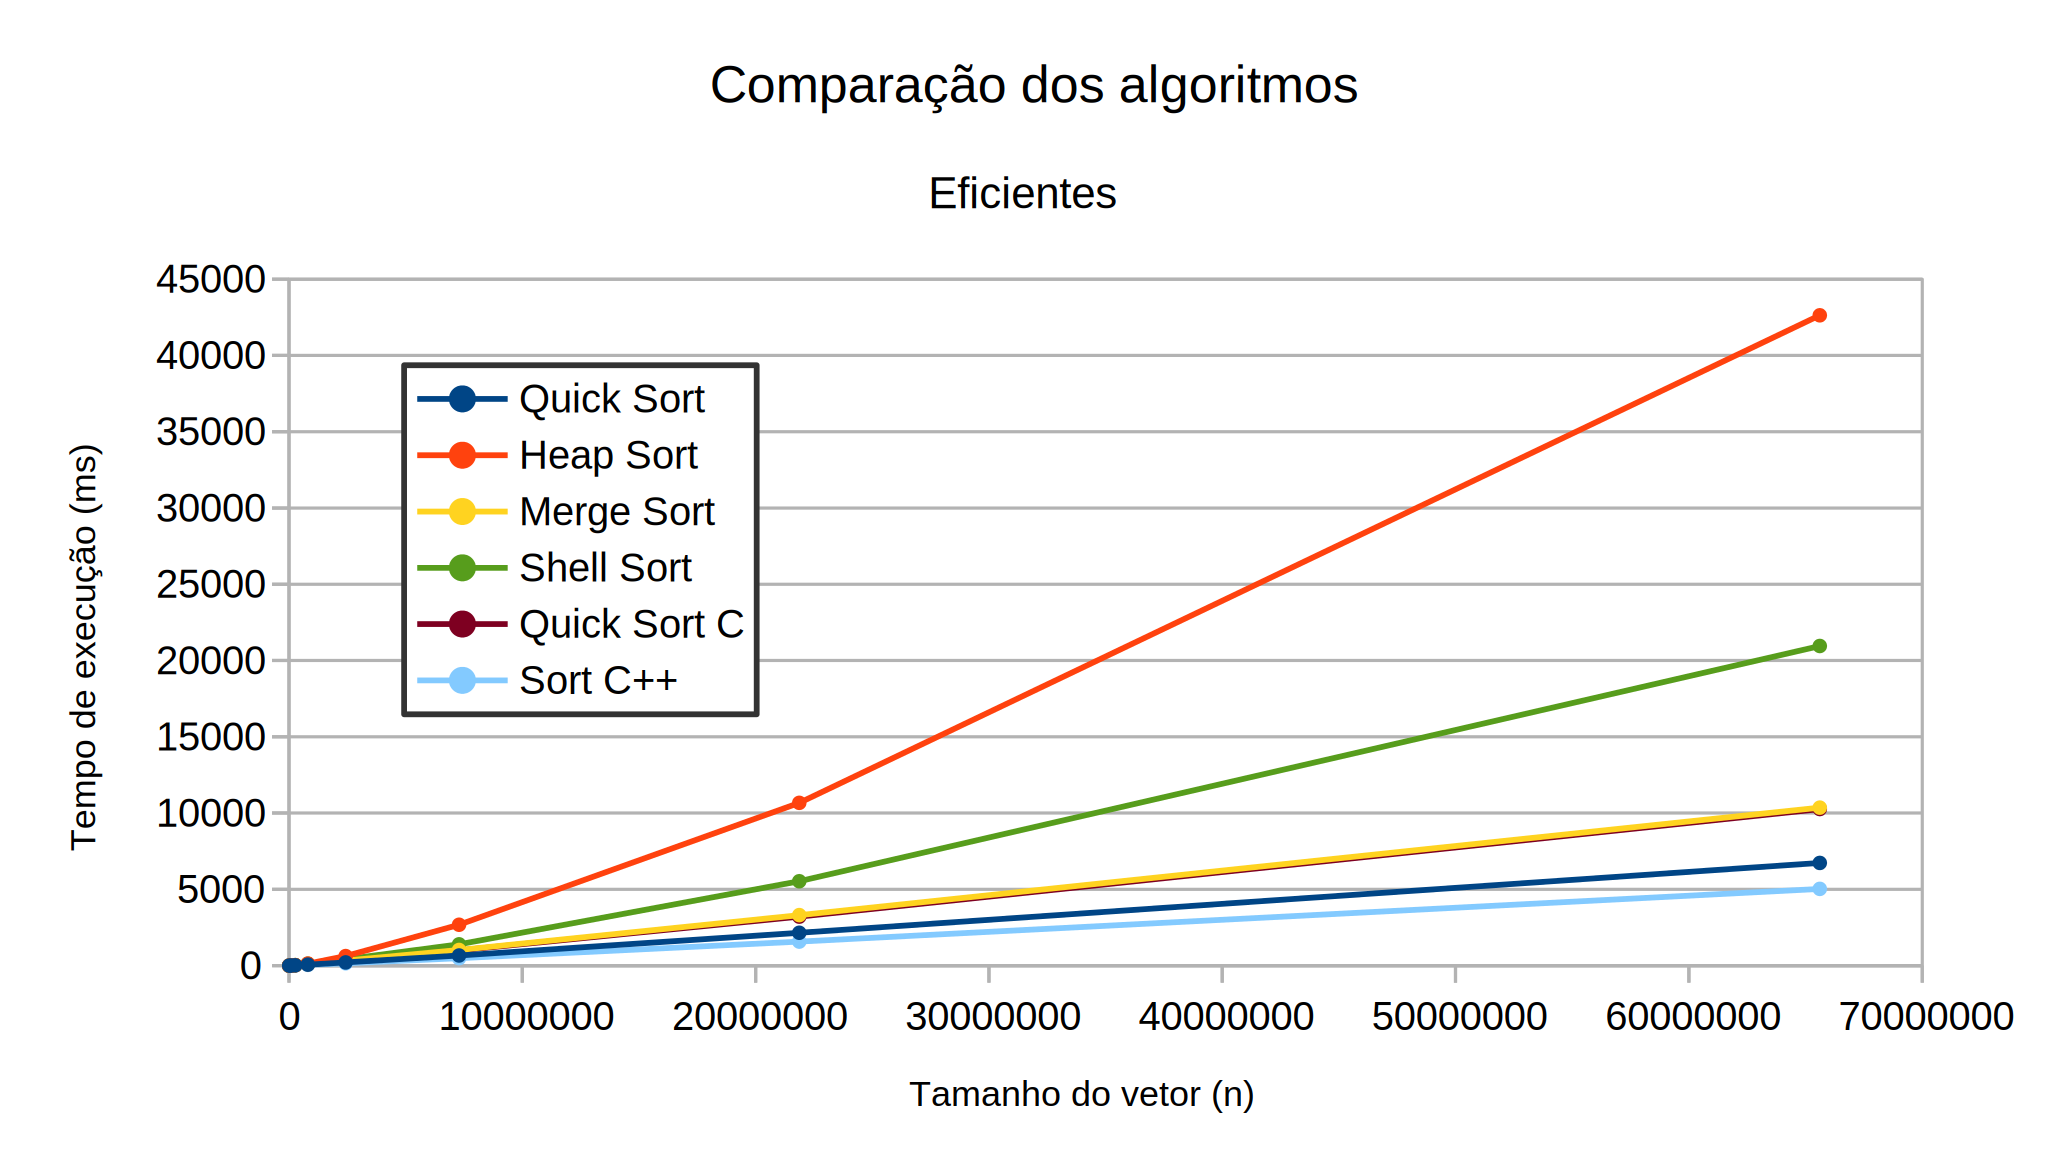
\includegraphics[width=10cm]{comp_efic.png}
	\caption[Comparação dos algoritmos eficientes.]
	{Comparação dos algoritmos eficientes.}
	\label{chart:comp_efic}
\end{figure}

\begin{figure}[hb]
	\centering
	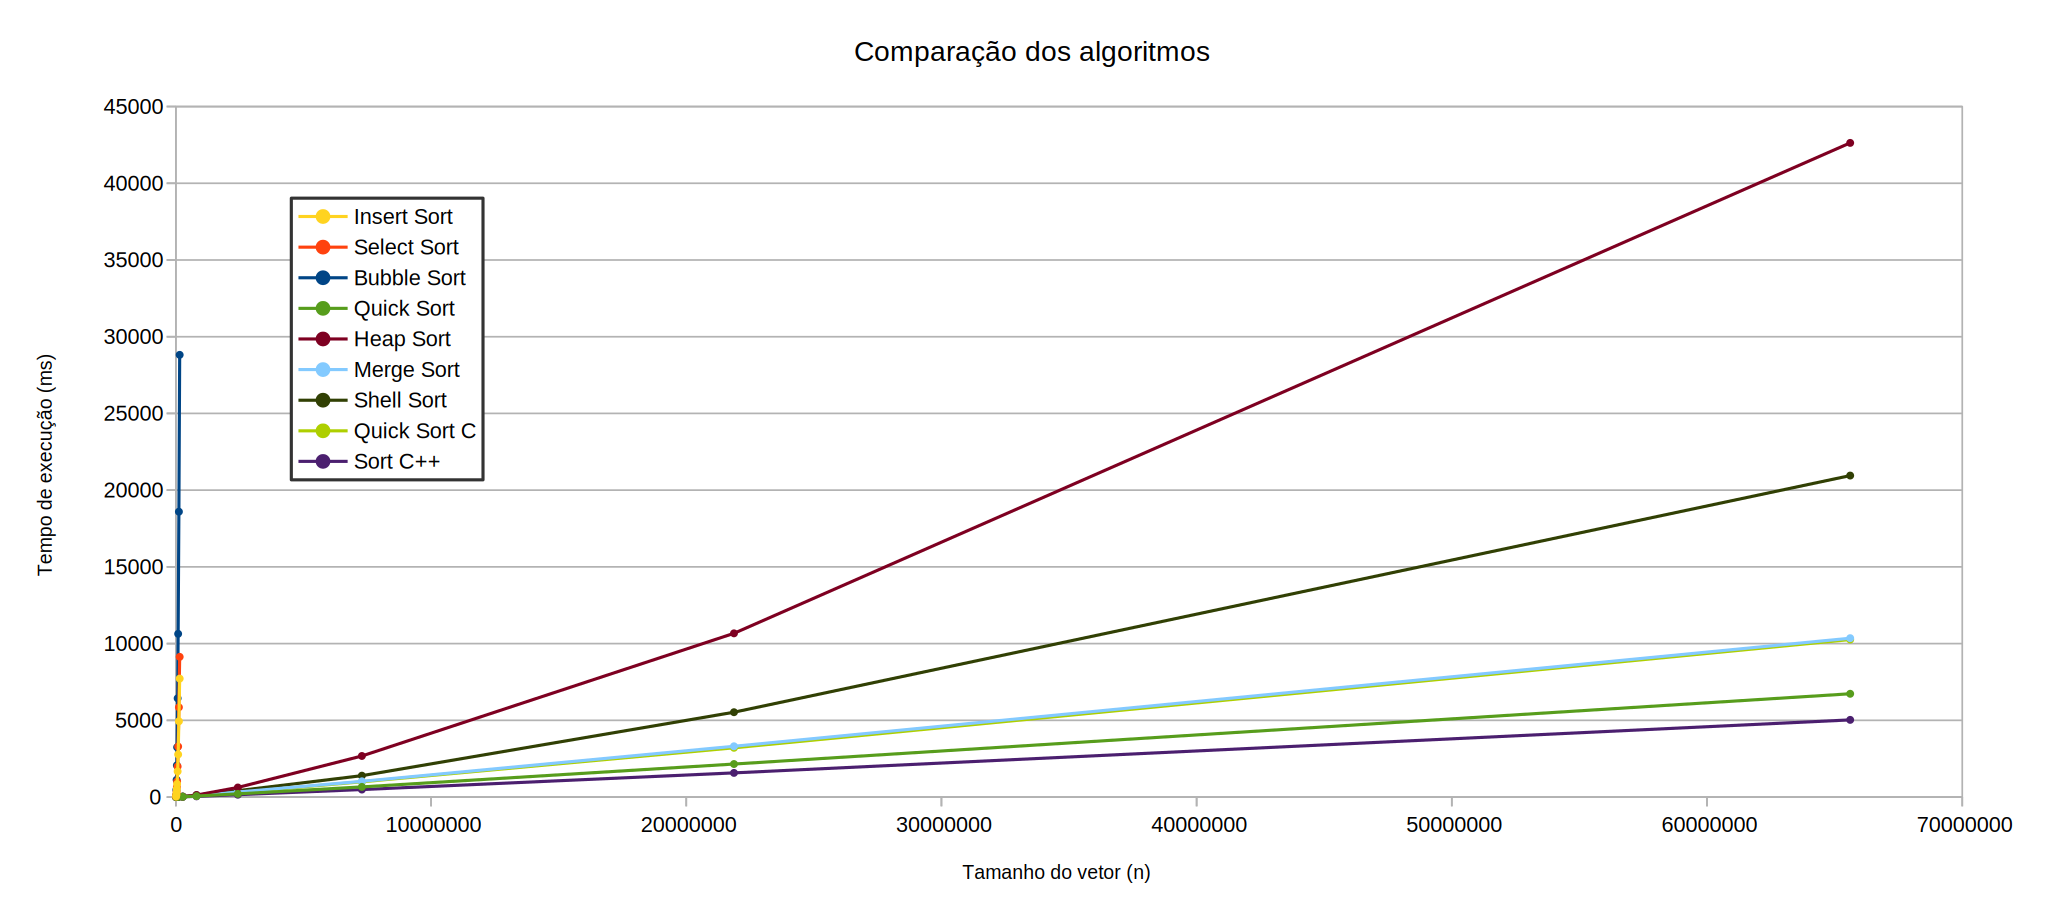
\includegraphics[width=16cm]{comp_todos.png}
	\caption[Comparação de todos os algoritmos.]
	{Comparação de todos os algoritmos.}
	\label{chart:comp_todos}
\end{figure}

\FloatBarrier
\noindent
\section{Conclusão}

\hfill

Dados todos os resultado obtidos com o projeto, percebemos que não necessariamente um algoritmo de pior caso $O(n \log{n})$ vai ser sempre melhor que os algoritmos de pior caso $O(n^2)$. O quicksort é o melhor exemplo disso: apesar dessa característica, ele mantém uma alta eficiência para diversos tamanhos de entrada e inclusive é utilizado como o algoritmo de ordenação nativo de diversas linguagens de programação. Fica claro que os melhores algoritmos são aqueles que fazem os elementos darem grandes saltos no vetor, realizando comparações e trocas entre elementos apenas quando necessário.

\newpage

\bibliographystyle{abbrv}
\bibliography{bibliografia}
\nocite{*}



\end{document}
